\begin{figure}[!htbp]\centering
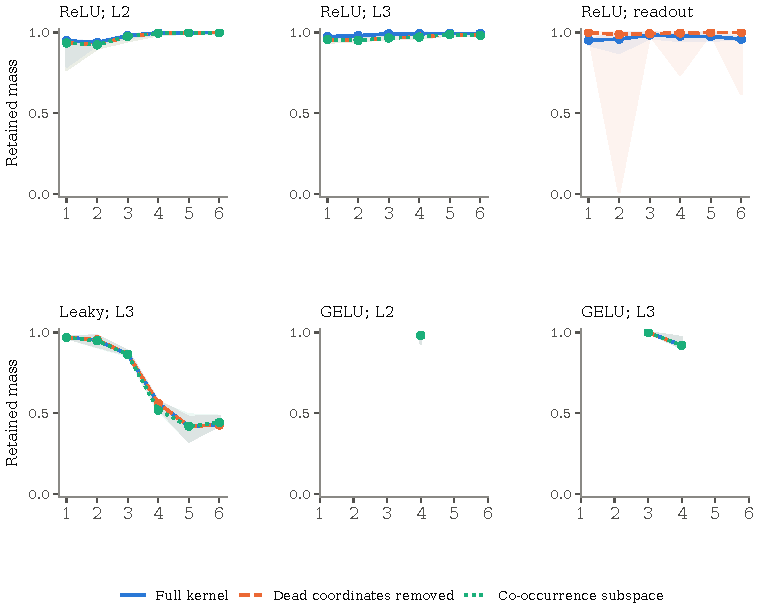
\includegraphics[width=4.560in]{persistence_summary_part1.pdf}
\caption{Checkpoint persistence in width-128 MNIST MLPs: retained mass. Pair indices 1--6 denote HA$\to$Int, Int$\to$100, 100$\to$250, 250$\to$500, HA$\to$500 and Int$\to$500; HA and Int are high accuracy and interpolation. Curves show medians and ranges across three seeds. Empty spaces have no retention value; unresolved component splits are omitted. GELU kernels remain cutoff-dependent.}\label{fig:persistence}
\end{figure}
\begin{figure}[!htbp]\centering
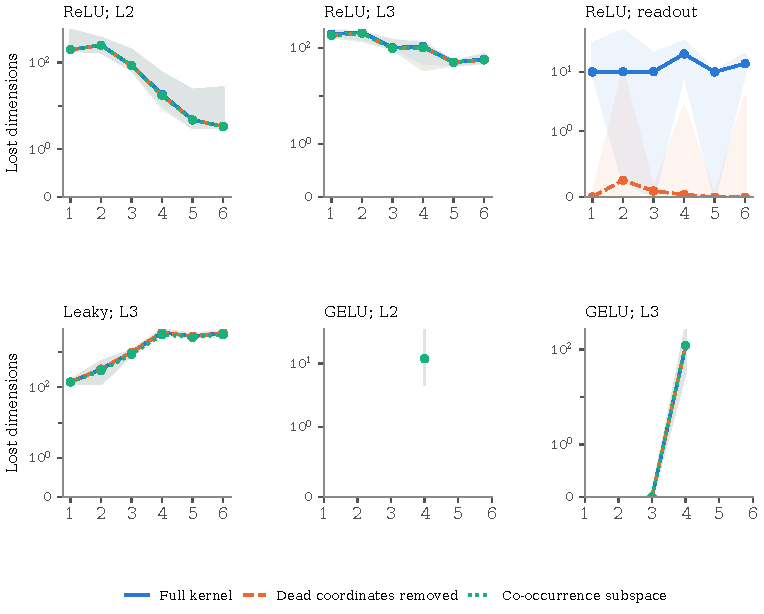
\includegraphics[width=4.583in]{persistence_summary_part2.pdf}
\caption{Effective lost dimension, with the checkpoint pairs and conventions of Figure~\ref{fig:persistence}. The vertical scale is linear near zero and logarithmic above it.}\label{fig:persistence-lost}
\end{figure}
\begin{figure}[!htbp]\centering
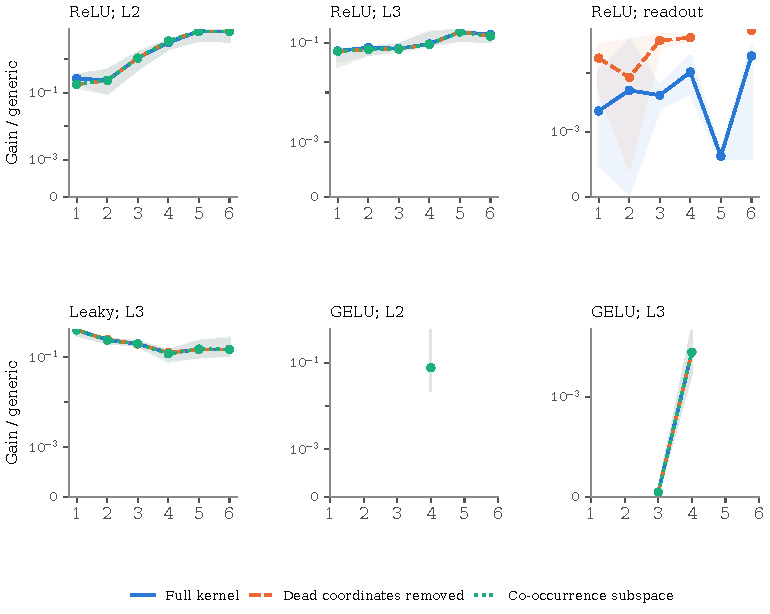
\includegraphics[width=4.620in]{persistence_summary_part3.pdf}
\caption{Output gain of lost components relative to generic directions, with the conventions of Figure~\ref{fig:persistence}.}\label{fig:persistence-gain}
\end{figure}
\begin{figure}[!htbp]\centering
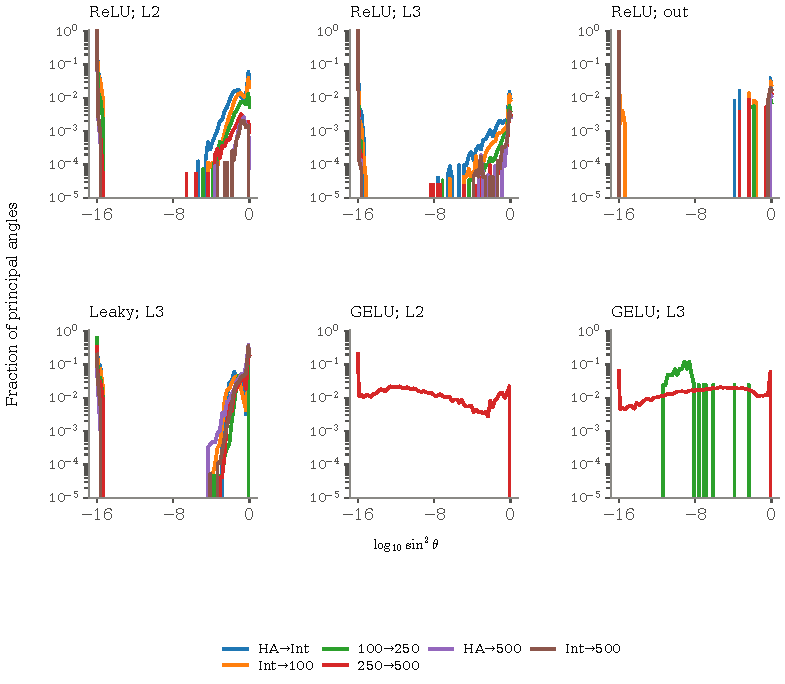
\includegraphics[width=4.710in]{persistence_angles.pdf}
\caption{Principal-angle distributions for the same checkpoint pairs, normalized within each seed and then averaged. ReLU retains a large aligned component, while leaky ReLU rotates more substantially late in training.}\label{fig:persistence-angles}
\end{figure}
\FloatBarrier
